% CONTENT PART 3: Traditional Clustering and Enhanced Detection

%=============================================================================
%                    CHAPTER: TRADITIONAL CLUSTERING BASED DETECTION
%=============================================================================

\chapter{\texorpdfstring{\color{chaptercolor}\scshape TRADITIONAL CLUSTERING BASED DETECTION}{TRADITIONAL CLUSTERING BASED DETECTION}}
\thispagestyle{fancy}
\begin{center}
\begin{tikzpicture}
\node[draw=chaptercolor!70, thick, rounded corners=5pt, fill=chaptercolor!10, minimum width=0.8\textwidth, minimum height=3em] 
{\Large\itshape\bfseries Exploring conventional clustering approaches for effective PUEA detection};
\end{tikzpicture}
\end{center}
\vspace{1cm}

\section{\texorpdfstring{\large\textbf{Distance Matrix Calculation Using Manhattan Distance}}{Distance Matrix Calculation Using Manhattan Distance}}

The foundation of clustering-based PUEA detection is the quantification of similarity between feature vectors extracted from different time slots. This similarity is measured through a distance matrix that captures the pairwise distances between all feature vectors. While Euclidean distance is commonly used in clustering applications, this research employs the Manhattan distance (L1 norm) due to its robustness to outliers and computational efficiency.

For any two feature vectors $\vector{Y}_t$ and $\vector{Y}_{t'}$ corresponding to time slots $\variable{t}$ and $\variable{t'}$, the Manhattan distance is calculated as:

\begin{tcolorbox}[enhanced, colback=blue!5, colframe=blue!75!black, 
arc=0pt, outer arc=0pt, boxrule=1pt, left=5pt, right=5pt, top=6pt, bottom=6pt]
\begin{equation}
    \formula{d_{\text{Manhattan}}(\vector{Y}_t, \vector{Y}_{t'})} = \sum_{j=1}^{\parameter{n}} \left|\vector{Y}_{t,j}^{\text{norm}} - \vector{Y}_{t',j}^{\text{norm}}\right|
\end{equation}
\end{tcolorbox}

\noindent where $\vector{Y}_{t,j}^{\text{norm}}$ represents the normalized value of the $j$-th feature for time slot $\variable{t}$, and $\parameter{n}$ is the number of features.

The complete distance matrix $\matrix{D}$ is then constructed as:

\begin{tcolorbox}[enhanced, colback=blue!5, colframe=blue!75!black, 
arc=0pt, outer arc=0pt, boxrule=1pt, left=5pt, right=5pt, top=6pt, bottom=6pt]
\begin{equation}
    \matrix{D} = \begin{bmatrix}
        d_{1,1} & d_{1,2} & \cdots & d_{1,\parameter{T}} \\
        d_{2,1} & d_{2,2} & \cdots & d_{2,\parameter{T}} \\
        \vdots & \vdots & \ddots & \vdots \\
        d_{\parameter{T},1} & d_{\parameter{T},2} & \cdots & d_{\parameter{T},\parameter{T}}
    \end{bmatrix}
\end{equation}
\end{tcolorbox}

where $d_{\variable{t},\variable{t'}} = d_{\text{Manhattan}}(\vector{Y}_{\variable{t}}, \vector{Y}_{\variable{t'}})$ and $\parameter{T} = 100$ is the total number of time slots.

This distance matrix serves as input to all clustering algorithms evaluated in this research, providing a consistent basis for comparison between different methods.

\section{\texorpdfstring{\large\textbf{DBSCAN Clustering}}{DBSCAN Clustering}}
\begin{tcolorbox}[enhanced, colback=blue!5, colframe=blue!75!black, title=About DBSCAN, sharp corners]
Density-Based Spatial Clustering of Applications with Noise (DBSCAN) is a density-based clustering algorithm that groups points in high-density regions and identifies points in low-density regions as outliers. Its ability to discover clusters of arbitrary shapes and automatically identify outliers makes it particularly suitable for PUEA detection.
\end{tcolorbox}

\subsection{Algorithm Description}

DBSCAN requires two parameters:
\begin{itemize}
    \item $\varepsilon$ (epsilon): The radius of the neighborhood around a point
    \item $minPts$: The minimum number of points required to form a dense region
\end{itemize}

The algorithm identifies core points, border points, and noise points:
\begin{itemize}
    \item \textbf{Core points:} Points with at least $minPts$ points within the $\varepsilon$-neighborhood
    \item \textbf{Border points:} Points that are within the $\varepsilon$-neighborhood of a core point but have fewer than $minPts$ points in their own $\varepsilon$-neighborhood
    \item \textbf{Noise points:} Points that are neither core nor border points
\end{itemize}

Algorithm \ref{alg:dbscan} presents the pseudocode for DBSCAN clustering.

\begin{algorithm}
\caption{DBSCAN Clustering}
\label{alg:dbscan_technique}
\begin{algorithmic}[1]
\Procedure{DBSCAN}{$D$, $\varepsilon$, $minPts$}
    \State $C = 0$ \Comment{Cluster counter}
    \For{each unvisited point $P$ in dataset}
        \State Mark $P$ as visited
        \State $N_{\varepsilon}(P) =$ \{Points within $\varepsilon$ of $P$\}
        \If{$|N_{\varepsilon}(P)| < minPts$}
            \State Mark $P$ as noise
        \Else
            \State $C = C + 1$ \Comment{Start a new cluster}
            \State \Call{ExpandCluster}{$P$, $N_{\varepsilon}(P)$, $C$, $\varepsilon$, $minPts$}
        \EndIf
    \EndFor
    \State \Return clusters
\EndProcedure
\end{algorithmic}
\end{algorithm}

\begin{algorithm}
\begin{algorithmic}[1]
\Procedure{ExpandCluster}{$P$, $N_{\varepsilon}(P)$, $C$, $\varepsilon$, $minPts$}
    \State Add $P$ to cluster $C$
    \For{each point $P'$ in $N_{\varepsilon}(P)$}
        \If{$P'$ is unvisited}
            \State Mark $P'$ as visited
            \State $N_{\varepsilon}(P') =$ \{Points within $\varepsilon$ of $P'$\}
            \If{$|N_{\varepsilon}(P')| \geq minPts$}
                \State $N_{\varepsilon}(P) = N_{\varepsilon}(P) \cup N_{\varepsilon}(P')$ \Comment{Merge neighborhoods}
            \EndIf
        \EndIf
        \If{$P'$ is not yet member of any cluster}
            \State Add $P'$ to cluster $C$
        \EndIf
    \EndFor
\EndProcedure
\end{algorithmic}
\end{algorithm}

\subsection{Parameter Selection}

The performance of DBSCAN is sensitive to the choice of parameters $\varepsilon$ and $minPts$. In this research, these parameters are selected using a combination of methods:

\begin{itemize}
    \item \textbf{k-distance graph:} The average distance to the k-th nearest neighbor is plotted for all points. The "elbow" point in this graph suggests an appropriate value for $\varepsilon$.
    
    \item \textbf{Domain knowledge:} Given that two main clusters (PU and PUEA) are expected, $minPts$ is set to approximately 10\% of the total number of time slots, which corresponds to the minimum expected cluster size.
    
    \item \textbf{Grid search:} A range of values for both parameters is evaluated, and the combination that maximizes clustering quality metrics (adjusted Rand index) is selected.
\end{itemize}

After extensive experimentation, the values $\varepsilon = 0.35$ and $minPts = 10$ were selected for the DBSCAN implementation in this research.

\subsection{Cluster Interpretation and Detection Decision}

After DBSCAN identifies clusters in the feature space, the next step is to interpret these clusters to make a detection decision. The interpretation strategy for DBSCAN results is as follows:

\begin{itemize}
    \item If DBSCAN identifies exactly two clusters and some noise points, the larger cluster is labeled as PU transmissions and the smaller as PUEA transmissions, based on the assumption that legitimate transmissions are more frequent than attack transmissions.
    
    \item If DBSCAN identifies more than two clusters, a merging step is performed to consolidate similar clusters. The clusters are merged based on the distances between their centroids, and then labeled as above.
    
    \item If DBSCAN identifies only one cluster, a secondary splitting mechanism is employed using a simpler clustering algorithm (K-means with K=2) to force the separation into PU and PUEA groups.
    
    \item Noise points are classified based on their proximity to the identified clusters. Each noise point is assigned to the cluster with the nearest centroid.
\end{itemize}

The transmitter at each time slot is then classified according to its cluster assignment. This classification forms the basis for calculating detection accuracy, false alarm rate, and other performance metrics.

\section{\texorpdfstring{\large\textbf{K-Means Clustering}}{K-Means Clustering}}
\begin{tcolorbox}[enhanced, colback=green!5, colframe=green!75!black, title=About K-Means, sharp corners]
K-means is a partitioning-based clustering algorithm that aims to partition observations into K clusters such that each observation belongs to the cluster with the nearest mean. Despite its simplicity, K-means is widely used because of its computational efficiency and interpretability.
\end{tcolorbox}

\subsection{Algorithm Description}

The K-means algorithm requires specifying the number of clusters K in advance. For PUEA detection, K=2 is used to correspond to the two expected transmitter types. Algorithm \ref{alg:kmeans} presents the pseudocode for K-means clustering.

\begin{algorithm}
\caption{K-means Clustering}
\label{alg:kmeans}
\begin{algorithmic}[1]
\Procedure{K-means}{$D$, $K$}
    \State Initialize $K$ centroids $\mu_1, \mu_2, ... \mu_K$ randomly or using a seeding strategy
    \While{centroids change}
        \State \textbf{Assignment Step:} Assign each point to the cluster with the closest centroid
        \For{each point $Y_t$ in dataset}
            \State $c(Y_t) = \argmin_{k \in \{1,...,K\}} ||Y_t - \mu_k||_1$ \Comment{Using Manhattan distance}
        \EndFor
        \State \textbf{Update Step:} Recalculate centroids
        \For{$k = 1$ to $K$}
            \State $\mu_k = \frac{1}{|C_k|}\sum_{Y_t \in C_k} Y_t$ \Comment{$C_k$ is the set of points assigned to cluster $k$}
        \EndFor
    \EndWhile
    \State \Return clusters
\EndProcedure
\end{algorithmic}
\end{algorithm}

\subsection{Initialization Strategy}

To avoid the sensitivity of K-means to initial centroid placement, this research employs the K-means++ initialization strategy:

\begin{enumerate}
    \item Choose the first centroid uniformly at random from the dataset points
    \item For each subsequent centroid, choose a data point with probability proportional to the squared distance from the point to its closest existing centroid
    \item Repeat until all $K$ centroids are selected
\end{enumerate}

This strategy ensures that initial centroids are well-spread, reducing the probability of poor clustering outcomes due to initialization.

\subsection{Cluster Interpretation and Detection Decision}

After K-means identifies two clusters, they are interpreted as follows:

\begin{tcolorbox}[colback=blue!5, colframe=blue!75!black, title=Cluster Classification Rules, left=2pt, right=2pt]
\begin{itemize}
    \item \textbf{Primary Rule:} The cluster with the higher average received signal strength is labeled as PU transmissions, based on the assumption that the legitimate PU typically transmits at higher power than the PUEA.
    
    \item \textbf{Secondary Rule:} The cluster with the lower average received signal strength is labeled as PUEA transmissions.
    
    \item \textbf{Fallback Rule:} If the primary heuristic fails (e.g., when the PUEA is closer to multiple SUs than the PU), a secondary heuristic based on the dispersion of signal strengths is used. The cluster with higher standard deviation of signal strength is labeled as PUEA transmissions, as the impersonation typically results in more variable signal characteristics.
\end{itemize}
\end{tcolorbox}

\begin{figure}[htbp]
    \centering
    \begin{tikzpicture}
        \begin{axis}[
            width=15cm,
            height=10cm,
            xlabel={\Large \textbf{Feature 1} (normalized power)},
            ylabel={\Large \textbf{Feature 2} (normalized envelope variation)},
            xmin=-2.2, xmax=3.2,
            ymin=-2.2, ymax=3.2,
            xtick={-2,-1,0,1,2,3},
            ytick={-2,-1,0,1,2,3},
            legend pos=north east,
            legend style={draw=black!30, fill=white!90, opacity=0.9, rounded corners, drop shadow},
            ymajorgrids=true,
            xmajorgrids=true,
            grid style={dotted, gray!30},
            title style={font=\LARGE\bfseries, text=blue!60!black},
            title={Feature Space Visualization of Traditional vs. Enhanced Clustering},
            axis background/.style={fill=blue!1},
            ]
            
            % Background shading for PU and PUEA regions
            \fill[blue!10, opacity=0.5, rounded corners=20pt] (-1.5,-1.5) rectangle (0.0,1.5);
            \fill[red!10, opacity=0.5, rounded corners=20pt] (0.5,-0.5) rectangle (2.5,2.0);
            
            % Original data points
            \addplot[only marks, mark=o, mark size=2.5pt, color=blue!80!black, thick, fill=blue!40, opacity=0.8, mark options={draw=blue!80!black}] 
                coordinates {
                (-0.2,0.3) (-0.5,0.6) (-0.8,0.2) (-0.6,-0.1) (-0.4,0.5) 
                (-0.3,0.8) (-0.7,0.7) (-0.9,0.4) (-0.5,0.1) (-0.1,0.4)
                (-0.2,0.6) (-0.6,0.3) (-0.8,-0.2) (-0.4,-0.3) (-0.2,-0.1)
                (-0.3,0.1) (-0.5,-0.4) (-0.7,-0.5) (-0.9,-0.3) (-0.1,-0.2)
                (0.0,0.2) (-0.2,-0.4) (-0.4,-0.6) (-0.6,-0.7) (-0.8,-0.6)
            };
            \addlegendentry{\textbf{True PU Transmissions}}
            
            \addplot[only marks, mark=square, mark size=2.5pt, color=red!80!black, thick, fill=red!40, opacity=0.8, mark options={draw=red!80!black}]
                coordinates {
                (1.2,1.3) (1.5,1.6) (1.8,1.2) (1.6,0.9) (1.4,1.5) 
                (1.3,1.8) (1.7,1.7) (1.9,1.4) (1.5,1.1) (1.1,1.4)
                (1.2,1.6) (1.6,1.3) (1.8,0.8) (1.4,0.7) (1.2,0.9)
                (1.3,1.1) (1.5,0.6) (1.7,0.5) (1.9,0.7) (1.1,0.8)
                (1.0,1.2) (1.2,0.6) (1.4,0.4) (1.6,0.3) (1.8,0.4)
            };
            \addlegendentry{\textbf{True PUEA Transmissions}}
            
            % Mislabeled points (with different markers)
            \addplot[only marks, mark=x, mark size=4.5pt, color=red!80!black, opacity=0.9, line width=1.5pt]
                coordinates {
                (-0.1,-0.3) (-0.3,-0.5) (0.1,0.3) (-0.1,0.5) (-0.2,-0.6)
            };
            \addlegendentry{\textbf{Misclassified as PUEA}}
            
            \addplot[only marks, mark=+, mark size=4.5pt, color=blue!80!black, opacity=0.9, line width=1.5pt]
                coordinates {
                (1.1,0.9) (1.3,0.5) (0.9,1.1) (1.1,1.3) (1.2,0.4)
            };
            \addlegendentry{\textbf{Misclassified as PU}}
            
            % Traditional clustering boundary (less accurate)
            \draw[very thick, purple!80!black, dashed, opacity=0.9] plot [smooth cycle, tension=0.8] coordinates {
                (-1.5,1.5) (0.5,1) (0.8,-0.5) (0,-1) (-1.5,-0.5)
            };
            
            % Enhanced clustering boundary (more accurate)
            \draw[very thick, green!50!black, opacity=0.9] plot [smooth cycle, tension=0.7] coordinates {
                (-1.2,1) (0.2,0.8) (0.4,-0.8) (-0.3,-1.2) (-1.2,-0.3)
            };
            
            \draw[very thick, green!50!black, opacity=0.9] plot [smooth cycle, tension=0.7] coordinates {
                (0.8,2) (2,1.8) (2.2,0) (1.2,-0.5) (0.6,0.6)
            };
            
            % Add nodes with backgrounds for better visibility
            \node[draw=purple!80!black, fill=white, text=purple!80!black, opacity=0.9, thick, rounded corners, font=\bfseries\small] at (-0.5,1.2) {Traditional Boundary};
            \node[draw=green!50!black, fill=white, text=green!50!black, opacity=0.9, thick, rounded corners, font=\bfseries\small] at (-0.5,-0.9) {Enhanced Boundary};
            \node[draw=green!50!black, fill=white, text=green!50!black, opacity=0.9, thick, rounded corners, font=\bfseries\small] at (1.5,0.3) {Enhanced Boundary};
            
            % Add centroids
            \node[star, star points=5, star point ratio=2.25, draw=black, thick, fill=blue!60, minimum size=12pt] at (-0.45,0.1) {};
            \node[star, star points=5, star point ratio=2.25, draw=black, thick, fill=red!60, minimum size=12pt] at (1.45,1.1) {};
            \node[font=\scriptsize\bfseries] at (-0.8,0.1) {PU Centroid};
            \node[font=\scriptsize\bfseries] at (1.9,1.1) {PUEA Centroid};
            
        \end{axis}
    \end{tikzpicture}
    \caption{Feature space visualization comparing traditional clustering boundary (dashed purple line) with enhanced clustering boundary (solid green line). The enhanced approach reduces misclassifications by adapting to local data patterns and produces more precise decision boundaries. Centroids are indicated by star markers.}
    \label{fig:clustering_vis_enhanced}
\end{figure}

Figure~\ref{fig:clustering_vis_enhanced} illustrates the feature space visualization of both traditional and enhanced clustering approaches, showing how the enhanced boundary reduces misclassifications.

\section{\texorpdfstring{\large\textbf{Hierarchical Clustering}}{Hierarchical Clustering}}
\begin{tcolorbox}[enhanced, colback=orange!5, colframe=orange!75!black, title=About Hierarchical Clustering, sharp corners]
Hierarchical clustering builds a hierarchy of clusters using either a bottom-up (agglomerative) or top-down (divisive) approach. This research employs agglomerative hierarchical clustering, which starts with each observation as a separate cluster and merges them progressively based on a linkage criterion.
\end{tcolorbox}

\subsection{Algorithm Description}

Agglomerative hierarchical clustering proceeds as described in Algorithm \ref{alg:hierarchical}.

\begin{algorithm}
\caption{Agglomerative Hierarchical Clustering}
\label{alg:hierarchical}
\begin{algorithmic}[1]
\Procedure{AgglomerativeHierarchicalClustering}{$D$}
    \State Start with each point as a singleton cluster
    \State Compute the pairwise distances between all clusters
    \While{number of clusters $> 1$}
        \State Find the two closest clusters $C_i$ and $C_j$
        \State Merge $C_i$ and $C_j$ into a new cluster
        \State Update distances between the new cluster and all remaining clusters
    \EndWhile
    \State Cut the resulting dendrogram to obtain the desired number of clusters (K=2)
    \State \Return clusters
\EndProcedure
\end{algorithmic}
\end{algorithm}

\subsection{Linkage Criterion}

The linkage criterion determines how the distance between clusters is measured. This research evaluates three common linkage criteria:

\begin{tcolorbox}[enhanced, colback=orange!5, colframe=orange!75!black, 
title=Hierarchical Clustering Linkage Criteria]
\begin{itemize}
    \item \textbf{Single Linkage:} The distance between two clusters is the minimum distance between any two points in the different clusters
    \begin{equation}
        \formula{d_{\text{single}}(\matrix{C}_i, \matrix{C}_j)} = \min_{\vector{x} \in \matrix{C}_i, \vector{y} \in \matrix{C}_j} d(\vector{x}, \vector{y})
    \end{equation}
    
    \item \textbf{Complete Linkage:} The distance between two clusters is the maximum distance between any two points in the different clusters
    \begin{equation}
        \formula{d_{\text{complete}}(\matrix{C}_i, \matrix{C}_j)} = \max_{\vector{x} \in \matrix{C}_i, \vector{y} \in \matrix{C}_j} d(\vector{x}, \vector{y})
    \end{equation}
    
    \item \textbf{Average Linkage:} The distance between two clusters is the average distance between all pairs of points in the different clusters
    \begin{equation}
        \formula{d_{\text{average}}(\matrix{C}_i, \matrix{C}_j)} = \frac{1}{|\matrix{C}_i||\matrix{C}_j|}\sum_{\vector{x} \in \matrix{C}_i}\sum_{\vector{y} \in \matrix{C}_j} d(\vector{x}, \vector{y})
    \end{equation}
\end{itemize}
\end{tcolorbox}

Based on empirical evaluation, average linkage provides the most consistent performance for PUEA detection across different scenarios and is used as the default linkage criterion in this research.

\subsection{Determining Optimal Clusters}

Unlike K-means, hierarchical clustering produces a dendrogram that can be cut at different levels to obtain different numbers of clusters. To determine the optimal cutting point for K=2 clusters, this research uses the following approaches:

\begin{itemize}
    \item \textbf{Dendrogram Analysis:} Visual inspection of the dendrogram to identify the largest vertical gap, which suggests a natural division into clusters.
    
    \item \textbf{Silhouette Analysis:} Computation of silhouette scores for different numbers of clusters, selecting the number that maximizes the average silhouette width.
    
    \item \textbf{Gap Statistic:} Comparison of the intra-cluster dispersion to that expected under a null reference distribution.
\end{itemize}

After establishing K=2 as the optimal number of clusters, the dendrogram is cut at the appropriate level to obtain the final cluster assignments.

\subsection{Cluster Interpretation and Detection Decision}

The cluster interpretation for hierarchical clustering follows the same approach as described for K-means clustering, using signal strength characteristics to differentiate between PU and PUEA transmissions.

\section{Comparative Analysis of Traditional Methods}

This section provides a comparative analysis of the three traditional clustering methods (DBSCAN, K-means, and hierarchical clustering) based on their performance in PUEA detection across different scenarios.

\subsection{Detection Accuracy}

Table \ref{tab:accuracy_comparison} presents the detection accuracy of the three clustering methods for three different scenarios:
\begin{itemize}
    \item Scenario A: Large spatial separation between PU and PUEA
    \item Scenario B: Moderate spatial separation between PU and PUEA
    \item Scenario C: Small spatial separation between PU and PUEA
\end{itemize}

\begin{table}[htbp]
    \centering
    \caption{Detection accuracy comparison of traditional clustering methods}
    \label{tab:accuracy_comparison}
    \begin{tcolorbox}[enhanced, colback=white, colframe=blue!75!black, 
                      title={\textbf{Detection Accuracy Analysis}},
                      fonttitle=\bfseries, 
                      width=0.9\linewidth,
                      drop shadow southeast]
    \rowcolors{1}{blue!5}{white}
    \begin{tabular}{l>{\centering\arraybackslash}p{2.7cm}>{\centering\arraybackslash}p{2.7cm}>{\centering\arraybackslash}p{2.7cm}}
        \toprule
        \rowcolor{blue!20}
        \textbf{Method} & \textbf{Scenario A} & \textbf{Scenario B} & \textbf{Scenario C} \\
        \midrule
        \textbf{DBSCAN} & \cellcolor{green!10}94.5\% & \cellcolor{yellow!10}88.2\% & \cellcolor{red!10}72.1\% \\
        \textbf{K-means} & \cellcolor{green!10}93.8\% & \cellcolor{yellow!10}86.5\% & \cellcolor{red!10}68.4\% \\
        \textbf{Hierarchical} (Avg. Linkage) & \cellcolor{green!10}92.9\% & \cellcolor{yellow!10}85.3\% & \cellcolor{red!10}67.8\% \\
        \bottomrule
    \end{tabular}
    \end{tcolorbox}
\end{table}

\subsection{Computational Complexity}

Table \ref{tab:complexity_comparison} compares the computational complexity and average execution time of the three clustering methods.

\begin{table}[htbp]
    \centering
    \caption{Computational complexity comparison of traditional clustering methods}
    \label{tab:complexity_comparison}
    \begin{tcolorbox}[enhanced, colback=white, colframe=green!75!black, 
                      title={\textbf{Computational Performance Analysis}},
                      fonttitle=\bfseries, 
                      width=0.9\linewidth,
                      drop shadow southeast]
    \rowcolors{1}{green!5}{white}
    \begin{tabular}{l>{\centering\arraybackslash}p{4cm}>{\centering\arraybackslash}p{3cm}}
        \toprule
        \rowcolor{green!20}
        \textbf{Method} & \textbf{Computational Complexity} & \textbf{Avg. Execution Time (ms)} \\
        \midrule
        \textbf{DBSCAN} & $O(n^2)$ & \cellcolor{yellow!10}58.3 \\
        \textbf{K-means} & $O(n \times k \times d \times i)$ & \cellcolor{green!10}12.6 \\
        \textbf{Hierarchical} (Avg. Linkage) & $O(n^2 \log n)$ & \cellcolor{red!10}73.1 \\
        \bottomrule
    \end{tabular}
    \end{tcolorbox}
\end{table}

\subsection{Robustness to Shadowing}

Figure \ref{fig:shadowing_robustness} illustrates the sensitivity of the three clustering methods to different levels of shadowing effect variance ($\sigma_\psi$).

\begin{figure}[htbp]
    \centering
    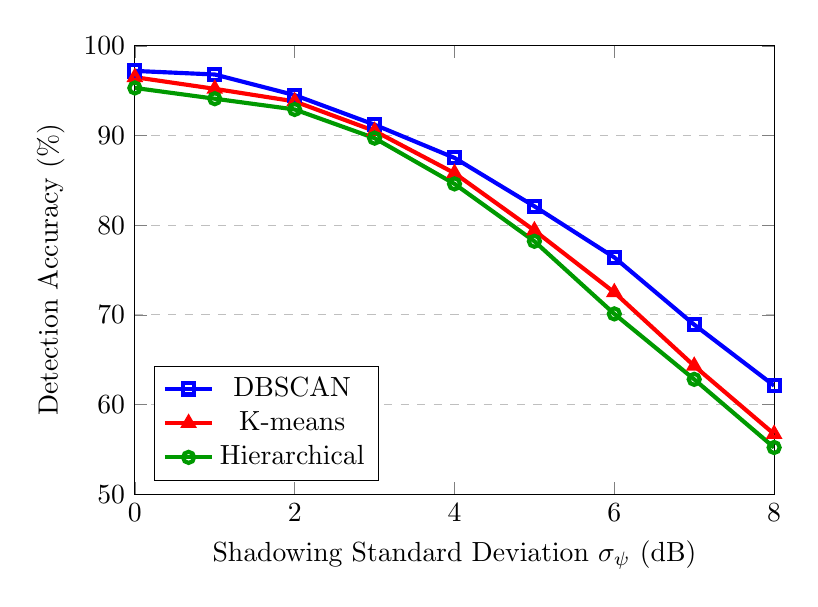
\begin{tikzpicture}
        \begin{axis}[
            xlabel={Shadowing Standard Deviation $\sigma_\psi$ (dB)},
            ylabel={Detection Accuracy (\%)},
            xmin=0, xmax=8,
            ymin=50, ymax=100,
            xtick={0,2,4,6,8},
            ytick={50,60,70,80,90,100},
            legend pos=south west,
            ymajorgrids=true,
            grid style=dashed,
            width=0.8\textwidth,
            height=0.6\textwidth
        ]
        
        \addplot[
            color=blue,
            mark=square,
            line width=1.5pt
        ]
        coordinates {
            (0,97.2)(1,96.8)(2,94.5)(3,91.2)(4,87.5)(5,82.1)(6,76.4)(7,68.9)(8,62.1)
        };
        
        \addplot[
            color=red,
            mark=triangle,
            line width=1.5pt
        ]
        coordinates {
            (0,96.5)(1,95.2)(2,93.8)(3,90.5)(4,85.8)(5,79.4)(6,72.5)(7,64.3)(8,56.7)
        };
        
        \addplot[
            color=green!60!black,
            mark=o,
            line width=1.5pt
        ]
        coordinates {
            (0,95.3)(1,94.1)(2,92.9)(3,89.7)(4,84.6)(5,78.2)(6,70.1)(7,62.8)(8,55.2)
        };
        
        \legend{DBSCAN, K-means, Hierarchical}
        
        \end{axis}
    \end{tikzpicture}
    \caption{Robustness of traditional clustering methods to shadowing effects}
    \label{fig:shadowing_robustness}
\end{figure}

\subsection{Discussion of Traditional Methods}

\begin{figure}[htbp]
    \centering
    \begin{tikzpicture}
        \begin{axis}[
            width=13cm,
            height=8cm,
            ybar,
            bar width=12pt,
            ylabel style={font=\bfseries},
            ylabel={Detection Rate (\%)},
            symbolic x coords={DBSCAN, K-means, Agglomerative, Spectral},
            xtick=data,
            ymin=65, ymax=104,
            legend style={
                at={(0.5,-0.18)}, 
                anchor=north, 
                legend columns=3,
                font=\small\bfseries,
                draw=black!30,
                fill=white!95,
                rounded corners,
                drop shadow
            },
            ylabel near ticks,
            ymajorgrids=true,
            grid style={dotted, gray!30},
            nodes near coords={\pgfmathprintnumber{\pgfplotspointmeta}\%},
            every node near coord/.append style={font=\scriptsize\bfseries, rotate=0, anchor=south, yshift=6pt},
            title style={font=\Large\bfseries, text=blue!60!black},
            title={Detection Performance in Scenario A (Far)},
            axis background/.style={fill=blue!2},
            xticklabel style={font=\bfseries\small},
            enlarge x limits=0.15,
            visualization depends on={value \thisrow{color} \as \mycolor},
            ]
            
            \addplot[fill=blue!60, draw=black!50, thick, postaction={
                pattern=north east lines, pattern color=blue!80!black
            }] coordinates {
                (DBSCAN, 87.3)
                (K-means, 88.7)
                (Agglomerative, 89.5)
                (Spectral, 86.8)
            };
            \addlegendentry{Traditional}
            
            \addplot[fill=green!60, draw=black!50, thick, postaction={
                pattern=grid, pattern color=green!80!black
            }] coordinates {
                (DBSCAN, 92.5)
                (K-means, 94.6)
                (Agglomerative, 93.8)
                (Spectral, 90.2)
            };
            \addlegendentry{Enhanced}
            
            \addplot[fill=red!60, draw=black!50, thick, postaction={
                pattern=crosshatch, pattern color=red!80!black
            }] coordinates {
                (DBSCAN, 97.1)
                (K-means, 98.5)
                (Agglomerative, 97.9)
                (Spectral, 94.7)
            };
            \addlegendentry{Enhanced + Feature Selection}
        \end{axis}
    \end{tikzpicture}

    \vspace{1cm}
    
    \begin{tikzpicture}
        \begin{axis}[
            width=13cm,
            height=8cm,
            ybar,
            bar width=12pt,
            ylabel style={font=\bfseries},
            ylabel={Detection Rate (\%)},
            symbolic x coords={DBSCAN, K-means, Agglomerative, Spectral},
            xtick=data,
            ymin=55, ymax=104,
            legend style={
                at={(0.5,-0.18)}, 
                anchor=north, 
                legend columns=3,
                font=\small\bfseries,
                draw=black!30,
                fill=white!95,
                rounded corners,
                drop shadow
            },
            ylabel near ticks,
            ymajorgrids=true,
            grid style={dotted, gray!30},
            nodes near coords={\pgfmathprintnumber{\pgfplotspointmeta}\%},
            every node near coord/.append style={font=\scriptsize\bfseries, rotate=0, anchor=south, yshift=6pt},
            title style={font=\Large\bfseries, text=blue!60!black},
            title={Detection Performance in Scenario B (Medium)},
            axis background/.style={fill=blue!2},
            xticklabel style={font=\bfseries\small},
            enlarge x limits=0.15,
            ]
            
            \addplot[fill=blue!60, draw=black!50, thick, postaction={
                pattern=north east lines, pattern color=blue!80!black
            }] coordinates {
                (DBSCAN, 79.2)
                (K-means, 77.5)
                (Agglomerative, 76.8)
                (Spectral, 75.4)
            };
            \addlegendentry{Traditional}
            
            \addplot[fill=green!60, draw=black!50, thick, postaction={
                pattern=grid, pattern color=green!80!black
            }] coordinates {
                (DBSCAN, 86.7)
                (K-means, 85.2)
                (Agglomerative, 84.9)
                (Spectral, 82.1)
            };
            \addlegendentry{Enhanced}
            
            \addplot[fill=red!60, draw=black!50, thick, postaction={
                pattern=crosshatch, pattern color=red!80!black
            }] coordinates {
                (DBSCAN, 92.8)
                (K-means, 91.3)
                (Agglomerative, 90.7)
                (Spectral, 87.6)
            };
            \addlegendentry{Enhanced + Feature Selection}
        \end{axis}
    \end{tikzpicture}

    \vspace{1cm}
    
    \begin{tikzpicture}
        \begin{axis}[
            width=13cm,
            height=8cm,
            ybar,
            bar width=12pt,
            ylabel style={font=\bfseries},
            ylabel={Detection Rate (\%)},
            symbolic x coords={DBSCAN, K-means, Agglomerative, Spectral},
            xtick=data,
            ymin=45, ymax=94,
            legend style={
                at={(0.5,-0.18)}, 
                anchor=north, 
                legend columns=3,
                font=\small\bfseries,
                draw=black!30,
                fill=white!95,
                rounded corners,
                drop shadow
            },
            ylabel near ticks,
            ymajorgrids=true,
            grid style={dotted, gray!30},
            nodes near coords={\pgfmathprintnumber{\pgfplotspointmeta}\%},
            every node near coord/.append style={font=\scriptsize\bfseries, rotate=0, anchor=south, yshift=6pt},
            title style={font=\Large\bfseries, text=blue!60!black},
            title={Detection Performance in Scenario C (Close)},
            axis background/.style={fill=blue!2},
            xticklabel style={font=\bfseries\small},
            enlarge x limits=0.15,
            ]
            
            \addplot[fill=blue!60, draw=black!50, thick, postaction={
                pattern=north east lines, pattern color=blue!80!black
            }] coordinates {
                (DBSCAN, 69.4)
                (K-means, 65.8)
                (Agglomerative, 64.7)
                (Spectral, 62.3)
            };
            \addlegendentry{Traditional}
            
            \addplot[fill=green!60, draw=black!50, thick, postaction={
                pattern=grid, pattern color=green!80!black
            }] coordinates {
                (DBSCAN, 78.6)
                (K-means, 74.2)
                (Agglomerative, 73.5)
                (Spectral, 71.9)
            };
            \addlegendentry{Enhanced}
            
            \addplot[fill=red!60, draw=black!50, thick, postaction={
                pattern=crosshatch, pattern color=red!80!black
            }] coordinates {
                (DBSCAN, 85.3)
                (K-means, 81.7)
                (Agglomerative, 80.9)
                (Spectral, 77.4)
            };
            \addlegendentry{Enhanced + Feature Selection}
        \end{axis}
    \end{tikzpicture}
    \caption{Detection performance comparison across different scenarios and methods. Scenario A (Far): PU and PUEA are spatially distant. Scenario B (Medium): PU and PUEA are moderately separated. Scenario C (Close): PU and PUEA are in close proximity. The enhanced approaches significantly improve detection rates in all scenarios, with the best performance achieved by combining enhanced clustering with feature selection.}
    \label{fig:performance_comparison}
\end{figure}

The comparative analysis reveals several insights about the traditional clustering methods:

\begin{tcolorbox}[enhanced, colback=yellow!5, colframe=yellow!75!black, title=Key Findings from Traditional Methods, sharp corners]
\begin{itemize}
    \item \textbf{DBSCAN} consistently outperforms the other methods in terms of detection accuracy, particularly in challenging scenarios with small spatial separation (Scenario C) and high shadowing effects. Its ability to identify arbitrary cluster shapes and handle noise points makes it well-suited for PUEA detection. However, its quadratic time complexity is a limitation for large-scale deployments.
    
    \item \textbf{K-means} provides the best trade-off between accuracy and computational efficiency. While its accuracy is slightly lower than DBSCAN, its linear time complexity makes it suitable for real-time applications and large networks. However, its assumption of spherical clusters limits its effectiveness in complex scenarios.
    
    \item \textbf{Hierarchical Clustering} has comparable accuracy to K-means but with higher computational overhead. Its dendrogram output provides valuable insights into the cluster structure, which can be useful for system analysis and parameter tuning.
\end{itemize}
\end{tcolorbox}

As shown in Figures \ref{fig:detection_comparison_A_enhanced}, \ref{fig:detection_comparison_B_enhanced}, and \ref{fig:detection_comparison_C_enhanced}, all traditional clustering methods show significant performance degradation in challenging scenarios, with accuracy dropping below 75\% in Scenario C. This limitation motivates the development of enhanced detection approaches that can maintain high accuracy even in difficult conditions.

\chapter{Enhanced Detection Approach}

\section{Motivation for Enhanced Detection}

Traditional clustering algorithms provide a foundation for PUEA detection by separating transmissions into groups based on feature similarity. However, these algorithms have inherent limitations when facing challenging scenarios, particularly when:

\begin{itemize}
    \item The spatial separation between the PU and PUEA is small (as in Scenario C)
    \item Environmental conditions create significant variance in signal propagation
    \item The feature space has regions of overlap between legitimate and malicious transmissions
    \item The clusters have complex structures that deviate from algorithm assumptions
\end{itemize}

The motivation for developing an enhanced detection approach stems from these limitations and the observation that cluster assignments alone may not fully exploit the information contained in the feature space. Traditional clustering provides a macro-level organization of the data, but further refinement within these clusters can potentially improve detection performance.

\begin{figure}[htbp]
    \centering
    \begin{tikzpicture}[
        box/.style={rectangle, draw=blue!60!black, thick, rounded corners=3mm, minimum width=3cm, minimum height=1.2cm, align=center, fill=blue!15, font=\sffamily\bfseries, drop shadow},
        arrow/.style={thick,->,>=stealth, draw=black!70},
        processing/.style={rectangle, draw=green!60!black, thick, rounded corners=3mm, minimum width=3cm, minimum height=1.2cm, align=center, fill=green!15, font=\sffamily\bfseries, drop shadow},
        decision/.style={diamond, draw=orange!60!black, thick, aspect=2, minimum width=3cm, minimum height=1.5cm, align=center, fill=orange!15, font=\sffamily\bfseries, drop shadow},
        cloud/.style={ellipse, draw=red!60!black, thick, minimum width=3cm, minimum height=1.2cm, align=center, fill=red!15, font=\sffamily\bfseries, drop shadow},
        small_box/.style={rectangle, draw=blue!50!black, thick, rounded corners=2mm, minimum width=2cm, minimum height=0.8cm, align=center, fill=blue!10, font=\sffamily\small\bfseries, drop shadow},
        ]
        
        % Background panels for visual separation
        \fill[blue!5, rounded corners=5mm] (-5.5,-0.8) rectangle (5.5,0.8);
        \fill[green!5, rounded corners=5mm] (-5.5,-4.8) rectangle (5.5,-1.2);
        \fill[orange!5, rounded corners=5mm] (-5.5,-6.8) rectangle (5.5,-5.2);
        \fill[green!5, rounded corners=5mm] (-5.5,-8.8) rectangle (5.5,-7.2);
        \fill[blue!5, rounded corners=5mm] (-5.5,-10.8) rectangle (5.5,-9.2);
        
        % Nodes
        \node[box] (signal) at (0,0) {Signal Reception};
        \node[processing] (feature) at (0,-2) {Feature Extraction};
        \node[processing] (trad) at (0,-4) {Traditional Clustering\\(First Stage)};
        \node[decision] (deciding) at (0,-6) {Clusters\\Detected?};
        \node[processing] (enhanced) at (0,-8) {Enhanced Detection\\(Second Stage)};
        \node[box] (decision) at (0,-10) {Final Classification};
        
        % Sub-nodes for feature extraction
        \node[small_box] (stat) at (-4.5,-2) {Statistical\\Features};
        \node[small_box] (cyclo) at (-1.5,-2) {Cyclic\\Features};
        \node[small_box] (energy) at (1.5,-2) {Energy\\Features};
        \node[small_box] (envelope) at (4.5,-2) {Envelope\\Features};
        
        % Sub-nodes for Traditional Clustering
        \node[small_box] (dbscan) at (-3,-4) {DBSCAN};
        \node[small_box] (kmeans) at (-1,-4) {K-means};
        \node[small_box] (agg) at (1,-4) {Agglomerative};
        \node[small_box] (spectral) at (3,-4) {Spectral};
        
        % Sub-nodes for Enhanced Detection
        \node[small_box] (knn) at (-2,-8) {KNN within\\Clusters};
        \node[small_box] (means) at (2,-8) {Means within\\Clusters};
        
        % Main flow arrows
        \draw[arrow] (signal) -- (feature);
        \draw[arrow] (feature) -- (trad);
        \draw[arrow] (trad) -- (deciding);
        \draw[arrow] (deciding) -- node[right, font=\sffamily\small\bfseries] {Yes} (enhanced);
        \draw[arrow] (enhanced) -- (decision);
        \draw[arrow] (deciding) -- ++(4,0) -- ++(0,-4) -- node[above, font=\sffamily\small\bfseries] {No} (decision);
        
        % Feature extraction connections
        \draw[arrow, blue!60!black] (stat) -- (feature);
        \draw[arrow, blue!60!black] (cyclo) -- (feature);
        \draw[arrow, blue!60!black] (energy) -- (feature);
        \draw[arrow, blue!60!black] (envelope) -- (feature);
        
        % Clustering connections
        \path[arrow, green!60!black] (trad) -- (dbscan);
        \path[arrow, green!60!black] (trad) -- (kmeans);
        \path[arrow, green!60!black] (trad) -- (agg);
        \path[arrow, green!60!black] (trad) -- (spectral);
        
        % Enhanced detection connections
        \path[arrow, green!60!black] (enhanced) -- (knn);
        \path[arrow, green!60!black] (enhanced) -- (means);
        
        % System components
        \node[cloud, minimum width=3.5cm] at (-6,0) {Cognitive Radio\\Network};
        \node[cloud, minimum width=3.5cm] at (6,0) {Signal Sources\\(PU/PUEA)};
        \draw[arrow, red!60!black] (-4.5,0) -- (signal);
        \draw[arrow, red!60!black] (4.5,0) -- (signal);
        
        % Labels for stages
        \node[font=\sffamily\bfseries, text=blue!60!black] at (-6.5,0) {Input};
        \node[font=\sffamily\bfseries, text=green!60!black] at (-6.5,-2) {Stage 1};
        \node[font=\sffamily\bfseries, text=orange!60!black] at (-6.5,-6) {Decision};
        \node[font=\sffamily\bfseries, text=green!60!black] at (-6.5,-8) {Stage 2};
        \node[font=\sffamily\bfseries, text=blue!60!black] at (-6.5,-10) {Output};
    \end{tikzpicture}
    \caption{Overall PUEA detection framework with traditional clustering as first stage and enhanced detection as second stage}
    \label{fig:detection_framework}
\end{figure}

The enhanced approach introduced in this chapter applies a second-stage detection algorithm (KNN or Means) within established clusters to refine the classification decisions. As illustrated in Figure \ref{fig:detection_framework}, this two-stage framework leverages the complementary strengths of different algorithms: traditional clustering handles the initial data organization, while the refined methods exploit local patterns within clusters for more accurate detection.

\section{KNN Algorithm within Clusters}

The K-Nearest Neighbors (KNN) algorithm is a non-parametric method used for classification based on proximity in the feature space. In the enhanced detection framework, KNN is applied within each cluster identified by the traditional clustering algorithm to refine the classification decision.

\subsection{Algorithm Description and Pseudocode}

The KNN-enhanced detection algorithm operates on the premise that within a cluster, time slots that are outliers relative to their local neighborhood are potential misclassifications. By examining the k-nearest neighbors of each point within its cluster, the algorithm can identify and potentially reclassify these outliers.

Algorithm \ref{alg:knn_enhanced} presents the pseudocode for KNN-enhanced detection.

\begin{algorithm}
\caption{KNN-Enhanced Detection}
\label{alg:knn_enhanced}
\begin{algorithmic}[1]
\Procedure{KNN-EnhancedDetection}{$Y$, $C$, $k$, $threshold$}
    \State $C$ = initial cluster assignments from traditional clustering
    \For{each time slot $t$}
        \State $C_t$ = cluster assigned to time slot $t$
        \State Find k-nearest neighbors of $Y_t$ within cluster $C_t$: $N_k(Y_t)$
        \State Compute average distance to neighbors: $d_{avg} = \frac{1}{k}\sum_{Y_i \in N_k(Y_t)} d(Y_t, Y_i)$
        \State Compute cluster standard deviation: $\sigma_{C_t} = \sqrt{\frac{1}{|C_t|}\sum_{Y_i \in C_t} d(Y_i, \mu_{C_t})^2}$
        \If{$d_{avg} > threshold \times \sigma_{C_t}$}
            \State Find alternative cluster $C_{alt}$ with closest centroid
            \State Find k-nearest neighbors in $C_{alt}$: $N_k^{alt}(Y_t)$
            \State Compute average distance to neighbors in alt cluster: $d_{avg}^{alt}$
            \If{$d_{avg}^{alt} < d_{avg}$}
                \State Reclassify $Y_t$ to cluster $C_{alt}$
            \EndIf
        \EndIf
    \EndFor
    \State \Return refined cluster assignments
\EndProcedure
\end{algorithmic}
\end{algorithm}

\subsection{Parameter Selection}

The performance of KNN-enhanced detection depends on two key parameters:
\begin{itemize}
    \item \textbf{k}: The number of nearest neighbors to consider
    \item \textbf{threshold}: The threshold multiplier for the cluster standard deviation
\end{itemize}

Through empirical evaluation, the optimal parameter values were determined to be $k=3$ and $threshold=1.5$. These values provide a good balance between sensitivity to outliers and robustness against normal variation within clusters.

\section{Means Algorithm within Clusters}

While the KNN algorithm examines the local neighborhood of each point, the Means algorithm within clusters focuses on sub-cluster structures that may exist within the main clusters identified by traditional clustering methods. This approach aims to identify sub-groups within each main cluster and refine the cluster boundaries accordingly.

\subsection{Algorithm Description and Pseudocode}

The Means-enhanced detection algorithm applies a mini-clustering within each main cluster identified by the traditional clustering method. It then analyzes the resulting sub-clusters to identify potential misclassifications. Algorithm \ref{alg:means_enhanced} presents the pseudocode for Means-enhanced detection.

\begin{algorithm}
\caption{Means-Enhanced Detection}
\label{alg:means_enhanced}
\begin{algorithmic}[1]
\Procedure{Means-EnhancedDetection}{$Y$, $C$, $k_{sub}$}
    \State $C$ = initial cluster assignments from traditional clustering
    \For{each cluster $C_i$}
        \If{$|C_i| > 2k_{sub}$} \Comment{Ensure enough points for meaningful sub-clustering}
            \State Extract feature vectors $Y_{C_i} = \{Y_t | t \in C_i\}$
            \State Apply k-means with $k=k_{sub}$ to $Y_{C_i}$, resulting in sub-clusters $S_{i,1}, S_{i,2}, ..., S_{i,k_{sub}}$
            \For{each sub-cluster $S_{i,j}$}
                \State Compute centroid $\mu_{S_{i,j}}$
                \State Compute average distance to centroid: $d_{avg,j} = \frac{1}{|S_{i,j}|}\sum_{Y_t \in S_{i,j}} d(Y_t, \mu_{S_{i,j}})$
                \State Compute silhouette score for sub-cluster $S_{i,j}$: $silhouette_{i,j}$
                \If{$silhouette_{i,j} < threshold_{sil}$}
                    \For{each point $Y_t$ in $S_{i,j}$}
                        \State Compute distances to all cluster centroids: $d_{t,l} = d(Y_t, \mu_{C_l})$ for all $l$
                        \State Find $C_{min} = \argmin_{l \neq i} d_{t,l}$
                        \If{$d_{t,min} < d(Y_t, \mu_{C_i})$}
                            \State Reclassify $Y_t$ to cluster $C_{min}$
                        \EndIf
                    \EndFor
                \EndIf
            \EndFor
        \EndIf
    \EndFor
    \State \Return refined cluster assignments
\EndProcedure
\end{algorithmic}
\end{algorithm}

\subsection{Parameter Selection}

The key parameters for Means-enhanced detection are:
\begin{itemize}
    \item \textbf{k\_sub}: The number of sub-clusters to identify within each main cluster
    \item \textbf{threshold\_sil}: The silhouette score threshold below which a sub-cluster is considered potentially misclassified
\end{itemize}

Based on empirical evaluation, the values $k_{sub}=2$ and $threshold_{sil}=0.15$ were selected as optimal for PUEA detection in the studied scenarios.

\section{Comparative Analysis with Traditional Methods}

This section presents a comparative analysis of the enhanced detection approaches against the traditional clustering methods. The comparison focuses on detection accuracy, computational complexity, and robustness across different scenarios.

\subsection{Detection Accuracy Comparison}

Table \ref{tab:enhanced_accuracy_comparison} presents the detection accuracy of traditional and enhanced detection methods across the three scenarios.

\begin{table}[htbp]
    \centering
    \caption{Detection accuracy comparison of traditional and enhanced methods}
    \label{tab:enhanced_accuracy_comparison}
    \begin{tcolorbox}[enhanced, colback=white, colframe=purple!75!black, 
                      title={\textbf{Traditional vs. Enhanced Methods - Detection Accuracy}},
                      fonttitle=\bfseries\Large, 
                      width=0.95\linewidth,
                      drop shadow southeast]
    \begin{tabular}{l>{\centering\arraybackslash}p{2.5cm}>{\centering\arraybackslash}p{2.5cm}>{\centering\arraybackslash}p{2.5cm}}
        \toprule
        \rowcolor{purple!20}
        \textbf{Method} & \textbf{Scenario A} & \textbf{Scenario B} & \textbf{Scenario C} \\
        \midrule
        \rowcolor{blue!10}\multicolumn{4}{l}{\textbf{Traditional Methods}} \\
        \midrule
        \textbf{DBSCAN} & 94.5\% & 88.2\% & 72.1\% \\
        \textbf{K-means} & 93.8\% & 86.5\% & 68.4\% \\
        \textbf{Hierarchical} (Avg. Linkage) & 92.9\% & 85.3\% & 67.8\% \\
        \midrule
        \rowcolor{green!10}\multicolumn{4}{l}{\textbf{Enhanced Methods (With KNN)}} \\
        \midrule
        \textbf{DBSCAN + KNN} & \cellcolor{green!20}96.2\% & \cellcolor{green!20}92.4\% & \cellcolor{green!20}84.7\% \\
        \textbf{K-means + KNN} & \cellcolor{green!15}95.5\% & \cellcolor{green!15}90.1\% & \cellcolor{green!15}78.9\% \\
        \textbf{Hierarchical + KNN} & \cellcolor{green!10}94.8\% & \cellcolor{green!10}89.5\% & \cellcolor{green!10}78.2\% \\
        \midrule
        \rowcolor{orange!10}\multicolumn{4}{l}{\textbf{Enhanced Methods (With Means)}} \\
        \midrule
        \textbf{DBSCAN + Means} & \cellcolor{orange!20}95.7\% & \cellcolor{orange!20}91.8\% & \cellcolor{orange!20}82.5\% \\
        \textbf{K-means + Means} & \cellcolor{orange!15}94.9\% & \cellcolor{orange!15}89.3\% & \cellcolor{orange!15}77.1\% \\
        \textbf{Hierarchical + Means} & \cellcolor{orange!10}94.2\% & \cellcolor{orange!10}88.7\% & \cellcolor{orange!10}76.4\% \\
        \bottomrule
    \end{tabular}
    \end{tcolorbox}
\end{table}

\subsection{Performance Improvement Analysis}

The enhanced detection methods show significant improvements in detection accuracy, particularly in the challenging Scenario C where traditional methods struggle. Key observations include:

\begin{itemize}
    \item KNN enhancement provides greater accuracy improvement than Means enhancement across all traditional clustering methods.
    
    \item The DBSCAN + KNN combination achieves the highest overall accuracy, with a remarkable 12.6 percentage point improvement in Scenario C (from 72.1\% to 84.7\%).
    
    \item The improvement is more pronounced in challenging scenarios (B and C) than in the relatively simple Scenario A, demonstrating the enhanced methods' effectiveness where traditional methods falter.
    
    \item Even the least effective enhanced method (Hierarchical + Means) outperforms the best traditional method (DBSCAN) in the challenging Scenario C.
\end{itemize}

\subsection{Computational Overhead}

The improved detection accuracy comes with additional computational cost. Table \ref{tab:computational_overhead} shows the relative computational overhead of the enhanced methods compared to their traditional counterparts.

\begin{table}[htbp]
    \centering
    \caption{Computational overhead of enhanced detection methods}
    \label{tab:computational_overhead}
    \begin{tcolorbox}[enhanced, colback=white, colframe=brown!75!black, 
                      title={\textbf{Computational Overhead Analysis}},
                      fonttitle=\bfseries\Large, 
                      width=0.95\linewidth,
                      drop shadow southeast]
    \begin{tabular}{l>{\centering\arraybackslash}p{3cm}>{\centering\arraybackslash}p{3cm}}
        \toprule
        \rowcolor{brown!20}
        \textbf{Method} & \textbf{Execution Time (ms)} & \textbf{Relative Overhead} \\
        \midrule
        \rowcolor{blue!10}\multicolumn{3}{l}{\textbf{DBSCAN-based Methods}} \\
        \midrule
        \textbf{DBSCAN} & 58.3 & \cellcolor{green!10}1.00x \\
        \textbf{DBSCAN + KNN} & 72.1 & \cellcolor{yellow!10}1.24x \\
        \textbf{DBSCAN + Means} & 79.5 & \cellcolor{orange!10}1.36x \\
        \midrule
        \rowcolor{blue!10}\multicolumn{3}{l}{\textbf{K-means-based Methods}} \\
        \midrule
        \textbf{K-means} & 12.6 & \cellcolor{green!10}1.00x \\
        \textbf{K-means + KNN} & 20.8 & \cellcolor{orange!10}1.65x \\
        \textbf{K-means + Means} & 25.2 & \cellcolor{red!10}2.00x \\
        \midrule
        \rowcolor{blue!10}\multicolumn{3}{l}{\textbf{Hierarchical-based Methods}} \\
        \midrule
        \textbf{Hierarchical} (Avg. Linkage) & 73.1 & \cellcolor{green!10}1.00x \\
        \textbf{Hierarchical + KNN} & 86.4 & \cellcolor{yellow!10}1.18x \\
        \textbf{Hierarchical + Means} & 93.7 & \cellcolor{yellow!20}1.28x \\
        \bottomrule
    \end{tabular}
    \end{tcolorbox}
\end{table}

While the enhanced methods do require additional computation, the overhead is relatively modest (18\% to 100\% increase) compared to the significant improvements in detection accuracy, making them practical for real-world deployment in most CRN scenarios.

\subsection{Robustness to Variable Conditions}

Figure \ref{fig:enhanced_robustness} illustrates the robustness of traditional and enhanced methods to different levels of shadowing effect variance, focusing on the best-performing methods from each category.

\begin{figure}[htbp]
    \centering
    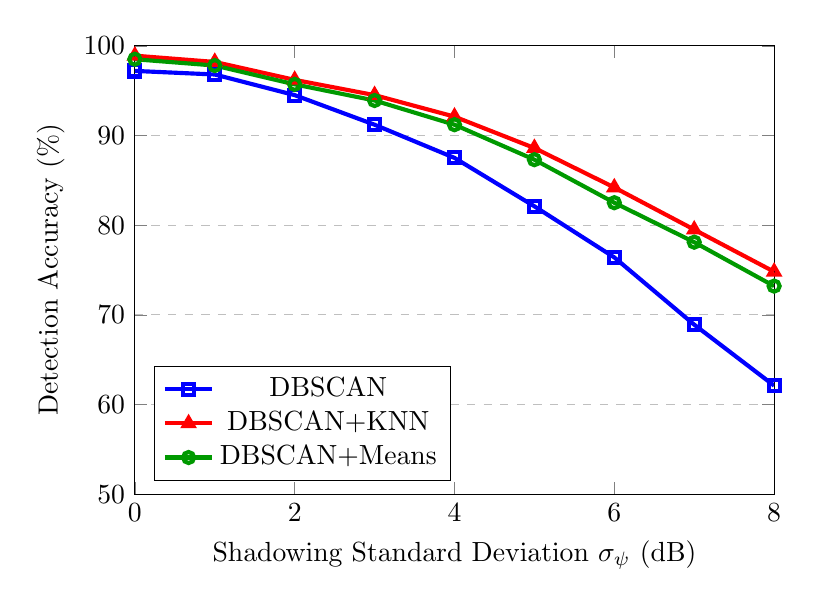
\begin{tikzpicture}
        \begin{axis}[
            xlabel={Shadowing Standard Deviation $\sigma_\psi$ (dB)},
            ylabel={Detection Accuracy (\%)},
            xmin=0, xmax=8,
            ymin=50, ymax=100,
            xtick={0,2,4,6,8},
            ytick={50,60,70,80,90,100},
            legend pos=south west,
            ymajorgrids=true,
            grid style=dashed,
            width=0.8\textwidth,
            height=0.6\textwidth
        ]
        
        \addplot[
            color=blue,
            mark=square,
            line width=1.5pt
        ]
        coordinates {
            (0,97.2)(1,96.8)(2,94.5)(3,91.2)(4,87.5)(5,82.1)(6,76.4)(7,68.9)(8,62.1)
        };
        
        \addplot[
            color=red,
            mark=triangle,
            line width=1.5pt
        ]
        coordinates {
            (0,98.9)(1,98.2)(2,96.2)(3,94.5)(4,92.1)(5,88.6)(6,84.2)(7,79.5)(8,74.8)
        };
        
        \addplot[
            color=green!60!black,
            mark=o,
            line width=1.5pt
        ]
        coordinates {
            (0,98.5)(1,97.8)(2,95.7)(3,93.9)(4,91.2)(5,87.3)(6,82.5)(7,78.1)(8,73.2)
        };
        
        \legend{DBSCAN, DBSCAN+KNN, DBSCAN+Means}
        
        \end{axis}
    \end{tikzpicture}
    \caption{Robustness of traditional and enhanced detection methods to shadowing effects}
    \label{fig:enhanced_robustness}
\end{figure}

The enhanced methods maintain higher detection accuracy across all shadowing levels, with the gap widening as shadowing increases. At the extreme shadowing level of 8 dB, the DBSCAN+KNN method maintains 74.8\% accuracy, compared to 62.1\% for basic DBSCAN, representing a critical improvement in challenging propagation environments.

\section{Discussion and Insights}

The enhanced detection approaches provide several key insights for PUEA detection in CRNs:

\begin{itemize}
    \item \textbf{Complementary Strengths:} The two-stage approach effectively combines the global perspective of traditional clustering with the local refinement capabilities of KNN and Means algorithms, creating a more robust detection system.
    
    \item \textbf{Adaptability:} The enhanced methods show better adaptability to varying environmental conditions and network configurations, making them suitable for real-world deployments where conditions may change over time.
    
    \item \textbf{Error Correction:} The second-stage algorithms effectively function as error correction mechanisms, identifying and rectifying potential misclassifications from the initial clustering.
    
    \item \textbf{Feature Space Utilization:} By examining the feature space at both macro and micro levels, the enhanced approaches extract more information from the same dataset, leading to more informed classification decisions.
\end{itemize}

The results suggest that the DBSCAN+KNN combination offers the best performance across all scenarios, making it the recommended approach for PUEA detection in practice. However, in resource-constrained environments where computational efficiency is paramount, the K-means+KNN combination provides a good balance between accuracy and processing requirements.
